\section{Equational reasoning}

\begin{frame}
    \frametitle{Now what?}

    We have a \alert{sound and complete} semantics for circuits as
    \alert{stream functions}.

    \wait

    But reasoning with streams can be a \alert{pain}...

    \wait
    Why not reason \alert{equationally}?
\end{frame}
\begin{frame}
    \frametitle{The two types of equation}

    \centering
    \begin{minipage}{0.49\textwidth}
        \centering
        \alert{Global}

        \vspace{1.5em}

        \dsptikzfig{strings/structure/cartesian/naturality-copy-lhs}[F][seq]
        =
        \dsptikzfig{strings/structure/cartesian/naturality-copy-rhs}[F][seq]
    \end{minipage}
    \begin{minipage}{0.49\textwidth}
        \centering
        \alert{Local}

        \vspace{1.5em}

        \dsptikzfig{circuits/axioms/fork-lhs}[v]
        =
        \dsptikzfig{circuits/axioms/fork-rhs}[v]
    \end{minipage}

    \vspace{1.5em}

    We want to stick to local equations \alert{as much as possible}.

\end{frame}

\begin{frame}
    \frametitle{What do the values do?}

    \centering
    \begin{axiom}
        \begin{minipage}{0.32\textwidth}
            \begin{equation*}
                \dsptikzfig{circuits/axioms/gate-lhs}
                =
                \dsptikzfig{circuits/axioms/gate-rhs-simple}
            \end{equation*}

            \visible<3->{
                \begin{equation*}
                    \dsptikzfig{circuits/axioms/join-lhs}[v][w]
                    =
                    \dsptikzfig{circuits/axioms/join-rhs}[v][w]
                \end{equation*}
            }
        \end{minipage}
        \begin{minipage}{0.32\textwidth}
            \visible<2->{
                \begin{equation*}
                    \dsptikzfig{circuits/axioms/fork-lhs}[v]
                    =
                    \dsptikzfig{circuits/axioms/fork-rhs}[v]
                \end{equation*}
            }

            \visible<4->{
                \begin{equation*}
                    \dsptikzfig{circuits/axioms/stub-lhs}[v]
                    =
                    \dsptikzfig{strings/monoidal/empty}
                \end{equation*}
            }
        \end{minipage}
        \begin{minipage}{0.32\textwidth}
            \visible<5->{
                \begin{equation*}
                    \dsptikzfig{circuits/axioms/disconnect-lhs}
                    =
                    \dsptikzfig{circuits/axioms/disconnect-rhs}
                \end{equation*}
            }
        \end{minipage}
    \end{axiom}

    \wait

    \visible<6->{
        For \(
            \dsptikzfig{circuits/components/values/v}[\overline{v}]
        \) and \(
            \dsptikzfig{strings/category/f}[F][comb]
        \), there exists \(
            \dsptikzfig{circuits/components/values/v}[\overline{w}]
        \) such that \(
            \dsptikzfig{circuits/components/circuits/f-applied}[F][comb][\overline{v}]
            =
            \dsptikzfig{circuits/components/values/v}[\overline{w}]
        \).
    }
\end{frame}
\begin{frame}
    \frametitle{Let's get structural}

    \centering
    \wait

    \((
        \dsptikzfig{strings/structure/monoid/merge}[comb],
        \dsptikzfig{strings/structure/monoid/init}[comb],
        \dsptikzfig{strings/structure/comonoid/copy}[comb],
        \dsptikzfig{strings/structure/comonoid/discard}[comb],
    )\) is a \alert{bialgebra}.
    \wait
    \begin{axiom}
        \centering
        \begin{minipage}{0.21\textwidth}
            \begin{equation*}
                \dsptikzfig{strings/structure/monoid/unitality-l-lhs}
                =
                \dsptikzfig{strings/structure/monoid/unitality-l-rhs}
            \end{equation*}
        \end{minipage}
        \quad
        \begin{minipage}{0.26\textwidth}
            \begin{equation*}
                \dsptikzfig{strings/structure/monoid/associativity-lhs}
                =
                \dsptikzfig{strings/structure/monoid/associativity-rhs}
            \end{equation*}
        \end{minipage}
        \quad
        \begin{minipage}{0.26\textwidth}
            \begin{equation*}
                \dsptikzfig{strings/structure/monoid/commutativity-lhs}
                =
                \dsptikzfig{strings/structure/monoid/commutativity-rhs}
            \end{equation*}
        \end{minipage}

        \begin{minipage}{0.21\textwidth}
            \begin{equation*}
                \dsptikzfig{strings/structure/comonoid/unitality-l-lhs}
                =
                \dsptikzfig{strings/structure/comonoid/unitality-l-rhs}
            \end{equation*}
        \end{minipage}
        \quad
        \begin{minipage}{0.26\textwidth}
            \begin{equation*}
                \dsptikzfig{strings/structure/comonoid/associativity-lhs}
                =
                \dsptikzfig{strings/structure/comonoid/associativity-rhs}
            \end{equation*}
        \end{minipage}
        \quad
        \begin{minipage}{0.26\textwidth}
            \begin{equation*}
                \dsptikzfig{strings/structure/comonoid/commutativity-lhs}
                =
                \dsptikzfig{strings/structure/comonoid/commutativity-rhs}
            \end{equation*}
        \end{minipage}

        \begin{minipage}{0.28\textwidth}
            \begin{equation*}
                \dsptikzfig{strings/structure/bialgebra/merge-copy-lhs}
                =
                \dsptikzfig{strings/structure/bialgebra/merge-copy-rhs}
            \end{equation*}
        \end{minipage}
        \begin{minipage}{0.23\textwidth}
            \begin{equation*}
                \dsptikzfig{strings/structure/bialgebra/init-copy-lhs}
                =
                \dsptikzfig{strings/structure/bialgebra/init-copy-rhs}
            \end{equation*}
        \end{minipage}
        \begin{minipage}{0.23\textwidth}
            \begin{equation*}
                \dsptikzfig{strings/structure/bialgebra/merge-discard-lhs}
                =
                \dsptikzfig{strings/structure/bialgebra/merge-discard-rhs}
            \end{equation*}
        \end{minipage}
        \begin{minipage}{0.2\textwidth}
            \begin{equation*}
                \dsptikzfig{strings/structure/bialgebra/init-discard-lhs}
                =
                \dsptikzfig{strings/structure/bialgebra/init-discard-rhs}
            \end{equation*}
        \end{minipage}
    \end{axiom}
\end{frame}
\begin{frame}
    \frametitle{Splitting things up}

    \centering

    \alert{Isolate} the sequential and combinational components...

    \wait
    \[
        \dsptikzfig{strings/category/f}[F][seq]
        =
        \dsptikzfig{circuits/productivity/pre-mealy-form-verbose}[F][s]
    \]

    \wait
    This is \emph{almost} another Mealy machine moment...
    \raisebox{-1.5em}{
        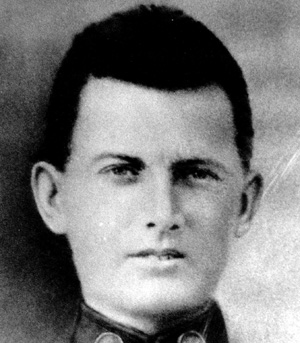
\includegraphics[width=0.1\textwidth]{imgs/mealy}
    }

    \wait
    ...but there is the non-delay-guarded trace!
\end{frame}
\begin{frame}
    \frametitle{Getting rid of non-delay-guarded feedback}

    \centering
    \[
        \dsptikzfig{circuits/instant-feedback/f0-box}
        :=
        \dsptikzfig{circuits/instant-feedback/f0-definition}
        \wait
        \qquad
        \dsptikzfig{circuits/instant-feedback/fkp1-box}
        :=
        \dsptikzfig{circuits/instant-feedback/fkp1-definition}
    \]

    \begin{axiom}
        \[
            \dsptikzfig{circuits/instant-feedback/equation-lhs}[F][][][x]
            \quad
            =
            \quad
            \dsptikzfig{circuits/instant-feedback/fixpoint-concrete}
        \]
    \end{axiom}

    \vspace{0.25em}

    \[
        \dsptikzfig{circuits/instant-feedback/trand}
        \quad
        =
        \quad
        \dsptikzfig{circuits/instant-feedback/trand-instfb}
    \]

\end{frame}
\begin{frame}
    \frametitle{Here's Mealy}

    \centering
    For \alert{any} circuit

    \[
        \dsptikzfig{strings/category/f}[F][seq]
        \quad
        =
        \quad
        \dsptikzfig{circuits/productivity/mealy-form-verbose}[F][s]
    \]

    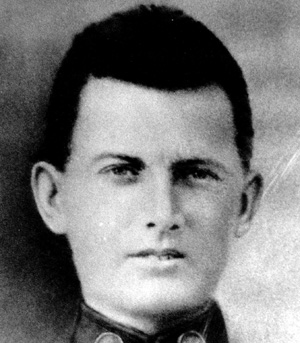
\includegraphics[width=0.25\textwidth]{imgs/mealy}

\end{frame}
\begin{frame}
    \frametitle{Let's get (even more) structural}

    What more structure can we add?

    \wait

    \alert{Forking} is natural...

    \wait

    \begin{axiom}
        \begin{minipage}{0.33\textwidth}
            \begin{equation*}
                \dsptikzfig{circuits/axioms/fork-gate-lhs}
                =
                \dsptikzfig{circuits/axioms/fork-gate-rhs}
            \end{equation*}
        \end{minipage}
        \begin{minipage}{0.33\textwidth}
            \begin{equation*}
                \dsptikzfig{circuits/axioms/fork-delay-lhs}
                =
                \dsptikzfig{circuits/axioms/fork-delay-rhs}
            \end{equation*}
        \end{minipage}
    \end{axiom}

    For any circuit...
    \(
        \dsptikzfig{strings/structure/cartesian/naturality-copy-lhs}[F][seq]
        =
        \dsptikzfig{strings/structure/cartesian/naturality-copy-rhs}[F][seq]
    \)
\end{frame}
\begin{frame}
    \frametitle{Let's (even even more) structural}

    Let's do the same for \alert{stubbing}...

    \begin{axiom}
        \begin{minipage}{0.22\textwidth}
            \begin{equation*}
                \dsptikzfig{circuits/axioms/stub-gate-lhs}
                =
                \dsptikzfig{circuits/axioms/stub-gate-rhs}
            \end{equation*}
        \end{minipage}
        \wait
        \begin{minipage}{0.2\textwidth}
            \begin{equation*}
                \dsptikzfig{circuits/axioms/unobservable-lhs}
                =
                \dsptikzfig{circuits/axioms/unobservable-rhs}
            \end{equation*}
        \end{minipage}
        \wait
        \quad
        \begin{minipage}{0.3\textwidth}
            \begin{equation*}
                \dsptikzfig{circuits/axioms/delay-discard-lhs}[F]
                =
                \dsptikzfig{circuits/axioms/delay-discard-rhs}
            \end{equation*}
        \end{minipage}
    \end{axiom}

    For any circuit...
    \(
        \dsptikzfig{strings/structure/cartesian/naturality-discard-lhs}[F][seq]
        =
        \dsptikzfig{strings/structure/cartesian/naturality-discard-rhs}
    \)

\end{frame}
\begin{frame}
    \frametitle{Let's get structural}

    \centering
    \[
        \dsptikzfig{strings/structure/cartesian/naturality-copy-lhs}[F][seq]
        =
        \dsptikzfig{strings/structure/cartesian/naturality-copy-rhs}[F][seq]
        \qquad
        \dsptikzfig{strings/structure/cartesian/naturality-discard-lhs}[F][seq]
        =
        \dsptikzfig{strings/structure/cartesian/naturality-discard-rhs}
    \]

    \LARGE
    \wait
    Cartesian!
    \normalsize
    \wait
    \[
        \dsptikzfig{strings/traced/trace-rhs}[F][seq]
        =
        \dsptikzfig{circuits/examples/reasoning/unfolding/unfolding-3}[F][seq]
    \]


\end{frame}
\begin{frame}
    \frametitle{Running the simulation}

    \centering

    \LARGE
    Goal:
    \normalsize

    \begin{equation*}
        \dsptikzfig{circuits/productivity/productive-goal-lhs-verbose}[F][v]
        =
        \dsptikzfig{circuits/productivity/productive-goal-rhs-verbose}[G][w]
    \end{equation*}

\end{frame}
\begin{frame}
    \frametitle{Running the simulation}

    \begin{axiom}
        \wait
        \[
            \dsptikzfig{circuits/axioms/streaming-lhs-verbose}[g][v]
            =
            \dsptikzfig{circuits/axioms/streaming-rhs}[g][v]
            \wait
            \qquad
            \dsptikzfig{circuits/axioms/join-delay-lhs}
            =
            \dsptikzfig{circuits/axioms/join-delay-rhs}
        \]
    \end{axiom}

    \[
        \dsptikzfig{circuits/axioms/generalised-streaming-lhs-verbose}[F][v]
        =
        \dsptikzfig{circuits/axioms/generalised-streaming-rhs}[F][v]
        =
        \dsptikzfig{circuits/axioms/generalised-streaming-rhs-reduced}[F][v]
    \]

\end{frame}
\begin{frame}
    \frametitle{Running the simulation}
    \[
        \dsptikzfig{circuits/productivity/productive-goal-lhs-verbose}[F][v]
        \wait
        =
        \dsptikzfig{circuits/productivity/productive-lhs-verbose}[F][v][s]
    \]

    \vspace{0.5em}
    \wait
    \(
        = \dsptikzfig{circuits/productivity/productive-step-9}[F][s][v]
    \)
    \wait
    \raisebox{-3em}{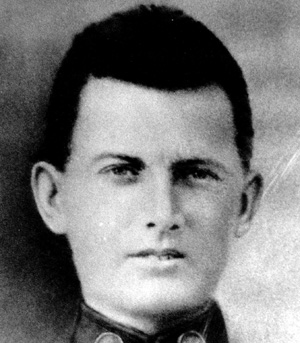
\includegraphics[width=0.2\textwidth]{imgs/mealy}}
\end{frame}